\documentclass[12pt]{article}\usepackage[]{graphicx}\usepackage[]{color}
% maxwidth is the original width if it is less than linewidth
% otherwise use linewidth (to make sure the graphics do not exceed the margin)
\makeatletter
\def\maxwidth{ %
  \ifdim\Gin@nat@width>\linewidth
    \linewidth
  \else
    \Gin@nat@width
  \fi
}
\makeatother

\definecolor{fgcolor}{rgb}{0.345, 0.345, 0.345}
\newcommand{\hlnum}[1]{\textcolor[rgb]{0.686,0.059,0.569}{#1}}%
\newcommand{\hlstr}[1]{\textcolor[rgb]{0.192,0.494,0.8}{#1}}%
\newcommand{\hlcom}[1]{\textcolor[rgb]{0.678,0.584,0.686}{\textit{#1}}}%
\newcommand{\hlopt}[1]{\textcolor[rgb]{0,0,0}{#1}}%
\newcommand{\hlstd}[1]{\textcolor[rgb]{0.345,0.345,0.345}{#1}}%
\newcommand{\hlkwa}[1]{\textcolor[rgb]{0.161,0.373,0.58}{\textbf{#1}}}%
\newcommand{\hlkwb}[1]{\textcolor[rgb]{0.69,0.353,0.396}{#1}}%
\newcommand{\hlkwc}[1]{\textcolor[rgb]{0.333,0.667,0.333}{#1}}%
\newcommand{\hlkwd}[1]{\textcolor[rgb]{0.737,0.353,0.396}{\textbf{#1}}}%
\let\hlipl\hlkwb

\usepackage{framed}
\makeatletter
\newenvironment{kframe}{%
 \def\at@end@of@kframe{}%
 \ifinner\ifhmode%
  \def\at@end@of@kframe{\end{minipage}}%
  \begin{minipage}{\columnwidth}%
 \fi\fi%
 \def\FrameCommand##1{\hskip\@totalleftmargin \hskip-\fboxsep
 \colorbox{shadecolor}{##1}\hskip-\fboxsep
     % There is no \\@totalrightmargin, so:
     \hskip-\linewidth \hskip-\@totalleftmargin \hskip\columnwidth}%
 \MakeFramed {\advance\hsize-\width
   \@totalleftmargin\z@ \linewidth\hsize
   \@setminipage}}%
 {\par\unskip\endMakeFramed%
 \at@end@of@kframe}
\makeatother

\definecolor{shadecolor}{rgb}{.97, .97, .97}
\definecolor{messagecolor}{rgb}{0, 0, 0}
\definecolor{warningcolor}{rgb}{1, 0, 1}
\definecolor{errorcolor}{rgb}{1, 0, 0}
\newenvironment{knitrout}{}{} % an empty environment to be redefined in TeX

\usepackage{alltt}
\usepackage{mathpazo}
\usepackage{hyperref,url}
\usepackage[a4paper,margin=1.5cm]{geometry}
\usepackage{listings}
\IfFileExists{upquote.sty}{\usepackage{upquote}}{}
\begin{document}


\title{A tutorial introduction to Make for reproducible research}
\author{Iain Davies and Daniel Nuest and Stephen J Eglen}

\date{\today}
\maketitle


\section{Introduction}





\section{Introduction}

Why make is useful.  Originally designed into 1970s for the efficient
compilation of programs.  Gradually adopted to other situations.


Note the workflow here

1. Generate
2. Analyse
3. Summarise


If Generating the data takes 10 hours, and analysing takes only 2
minutes, you don't want to rerun whole pipeline to regenerate data.


\section{Example problem}


\subsection{Estimating pi}

A useful example for using Make is the dartboard method for estimating pi.

Consider a dartboard of radius 1 set in a square of side length 2. We randomly throw darts uniformly across the square and count the fraction that land in the dartboard. In expectation, this fraction will be the ratio of the area of the dartboard (pi) to the area of the square (4). Hence we estimate pi as 4 times the fraction of darts that land in the dartboard. We may also want to display the position of the darts in a diagram for the ease of future readers.

We can write programs for this process which neatly capture the three steps of workflow above:
\begin{enumerate}
  \item Generating data. This is throwing the darts at the square and storing the position of each in an accesible format.
  \begin{itemize}
    \item inputs.dat - a file that states \emph{n}, the number of darts to be thrown.
    \item throw-darts.R - a R script that reads \emph{n} from inputs.dat and outputs a list of the positions of \emph{n} randomly thrown darts which is written to darts.xy.
    \item darts.xy - the list of positions of \emph{n} darts outputted by throw-darts.R.
  \end{itemize}
  \item Analysis. This is calculating the fraction of the darts which landed inside the dartboard and inferring an estimate of pi.
  \begin{itemize}
    \item count-inside.R - a R script that reads the position of each dart from darts.xy and writes whether it is inside the dartboard to inside.out.
    \item inside.out - a list of logicals corresponding to whether each dart is inside the dartboard.
    \item estimate.R - a R script that calculates an estimate of pi inferred from the list in inside.out. The estimate is written to pi.est.
    \item pi.est - a file containing the estimate of pi .
  \end{itemize}
  \item Summary. This is displaying the position of our thrown darts and our estimate of pi in an easily readable diagram.
  \begin{itemize}
    \item draw-figure.R - a R script that creates a diagram of the positions of the darts and estimate of pi and saves it to darts.pdf.
    \item darts.pdf - a diagram displaying the darts and estimate of pi.
  \end{itemize}
\end{enumerate}

We can use Make to execute these programs in the correct order and without repeating steps that haven't changed.

\subsection{Traditional approach - write a batch file}



\lstset{language=sh}
\fbox{\lstinputlisting{v1-R/pi-workflow.sh}}

\subsection{Version 1 (R makefile)}


\fbox{\lstinputlisting{v1-R/Makefile}}\\

The above is a simple Makefile that does the job. So how does it work?\\

\subsubsection{Anatomy of a Rule}

A Makefile is a list of instructions of how to create files in a process. It does this via \emph{rules}. \emph{Rules} consist of a \emph{target} file to be made, its \emph{dependencies} and finally a \emph{recipe} to make the target. For example, take the \emph{rule} for darts.xy above:\\
\fbox{\lstinputlisting[linerange={5-6}]{v1-R/Makefile}}\\

The \emph{target} is darts.xy. This is followed by a colon then a list of \emph{dependencies} - inputs.dat and throw−darts.R - which are the files needed to make darts.xy. Finally, the second line starts with a tab and then gives the \emph{recipe} to make darts.xy. This is a command run in the terminal - in this case executing the R file throw-darts.R with input input.dat and piping the output into darts.xy.\\

A \emph{rule} must be given for all files that are created in the process. For example, the Makefile above also gives \emph{rules} for inside.out (a list of whether the darts are inside the dartboard), pi.est (our esimate for pi) and darts.pdf (the diagram of thrown darts).

\subsection{Making Files - Importance of Dependencies}

If a file has a rule in the Makefile it can be made from the command line by executing "make $<$filename$>$". For example we can execute the recipe to make darts.xy by typing the following:

\begin{knitrout}
\definecolor{shadecolor}{rgb}{0.969, 0.969, 0.969}\color{fgcolor}\begin{kframe}
\begin{alltt}
cd v1-R
make darts.xy
\end{alltt}

\begin{verbatim}
## make[1]: Entering directory '/mhome/damtp/s/id318/Documents/Make_tutorial/make-tutorial/v1-R'
## Rscript throw-darts.R inputs.dat > darts.xy
## make[1]: Leaving directory '/mhome/damtp/s/id318/Documents/Make_tutorial/make-tutorial/v1-R'
\end{verbatim}
\end{kframe}
\end{knitrout}

This executes the recipe in the command line and produces the file darts.xy as desired. 

The clever part of the Make rule structure is that it determines whether a file should be remade by looking at the timestamps of the dependencies. If we repeat this command without changing any of the dependencies then Make will simply say that nothing is to be done:

\begin{knitrout}
\definecolor{shadecolor}{rgb}{0.969, 0.969, 0.969}\color{fgcolor}\begin{kframe}
\begin{alltt}
cd v1-R
make darts.xy
\end{alltt}

\begin{verbatim}
## make[1]: Entering directory '/mhome/damtp/s/id318/Documents/Make_tutorial/make-tutorial/v1-R'
## make[1]: 'darts.xy' is up to date.
## make[1]: Leaving directory '/mhome/damtp/s/id318/Documents/Make_tutorial/make-tutorial/v1-R'
\end{verbatim}
\end{kframe}
\end{knitrout}

This is the importance of dependencies - \underline{a target will only be remade if at least one of its dependencies has a more recent timestamp}. Furthermore, before making the target Make will remake any of its dependencies if their own dependencies have a more recent timestamp and so on.

\subsection{.PHONY targets}


\subsection{Running it (for real)}


\begin{knitrout}
\definecolor{shadecolor}{rgb}{0.969, 0.969, 0.969}\color{fgcolor}\begin{kframe}
\begin{alltt}
cd v1-R
make
\end{alltt}

\begin{verbatim}
## make[1]: Entering directory '/mhome/damtp/s/id318/Documents/Make_tutorial/make-tutorial/v1-R'
## Rscript count-inside.R darts.xy > inside.out
## Rscript estimate.R inside.out > pi.est
## Rscript draw-figure.R darts.xy inside.out pi.est darts.pdf
## make[1]: Leaving directory '/mhome/damtp/s/id318/Documents/Make_tutorial/make-tutorial/v1-R'
\end{verbatim}
\end{kframe}
\end{knitrout}

This should generate a new pdf, `darts.pdf`.  If we then delete
darts.pdf by accident, when we run `make` again, it will not need to
run all steps of the analysis, as the intermediate files are still
present.


\begin{knitrout}
\definecolor{shadecolor}{rgb}{0.969, 0.969, 0.969}\color{fgcolor}\begin{kframe}
\begin{alltt}
cd v1-R
rm darts.pdf
make
\end{alltt}

\begin{verbatim}
## make[1]: Entering directory '/mhome/damtp/s/id318/Documents/Make_tutorial/make-tutorial/v1-R'
## Rscript draw-figure.R darts.xy inside.out pi.est darts.pdf
## make[1]: Leaving directory '/mhome/damtp/s/id318/Documents/Make_tutorial/make-tutorial/v1-R'
\end{verbatim}
\end{kframe}
\end{knitrout}



\begin{figure}
  \centering
	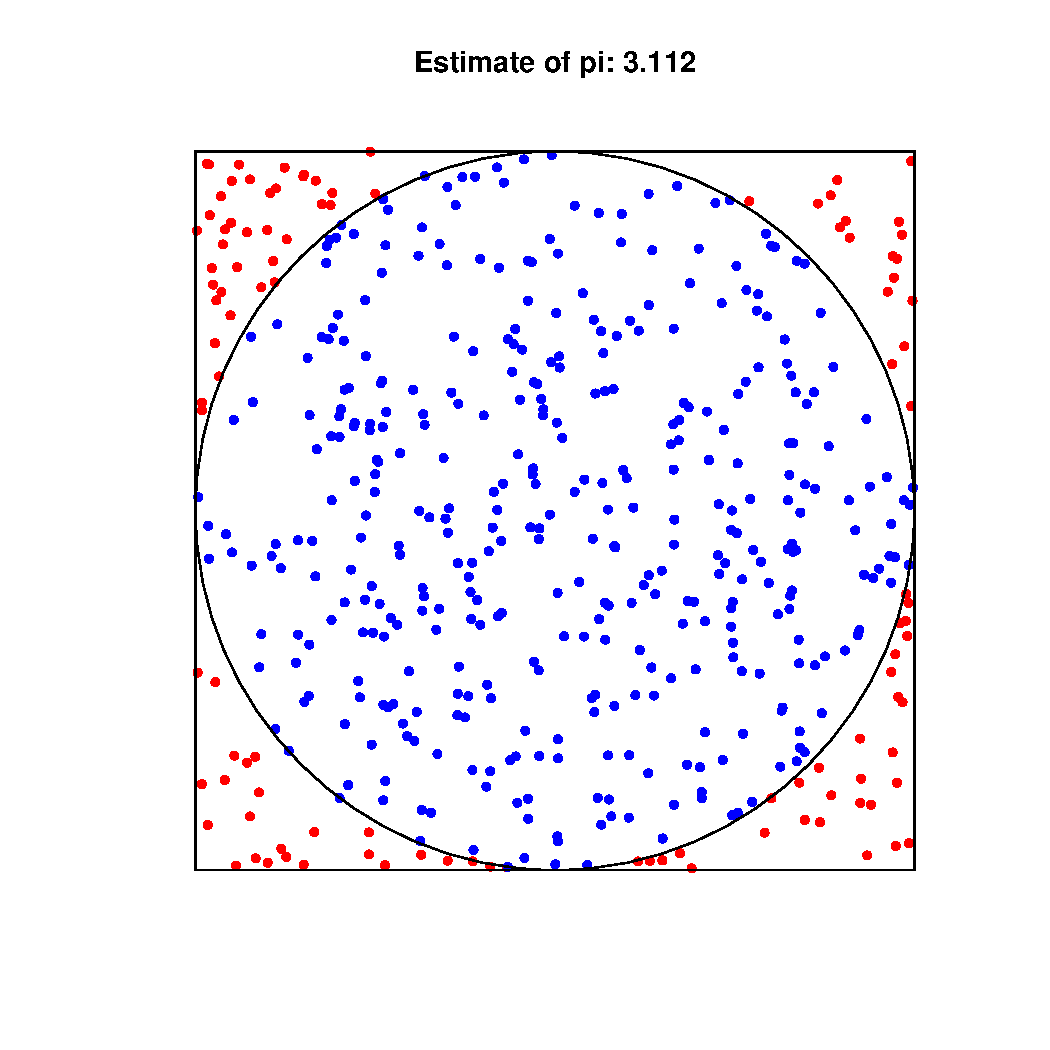
\includegraphics{v1-R/darts.pdf}
  \caption{Example output file, darts.pdf, created by "make" command.
  Blue (or red) points are those that were determined to be inside (or
  outside) the circle.  The estimate of pi, given in the title, was
  then given as 4*d/n, where d is the number of darts inside the
  circle and n is the total number of darts thrown.}
  \label{fig:darts}
\end{figure}



\subsection{DAG}

One nice thing about using a Makefile is usually you can visualize the
dependency graph.  e.g.  Figure~\ref{fig:dag}.  Input files are
clearly shown in green, and everything else in red can be regenerated.


\begin{figure}
  \centering
	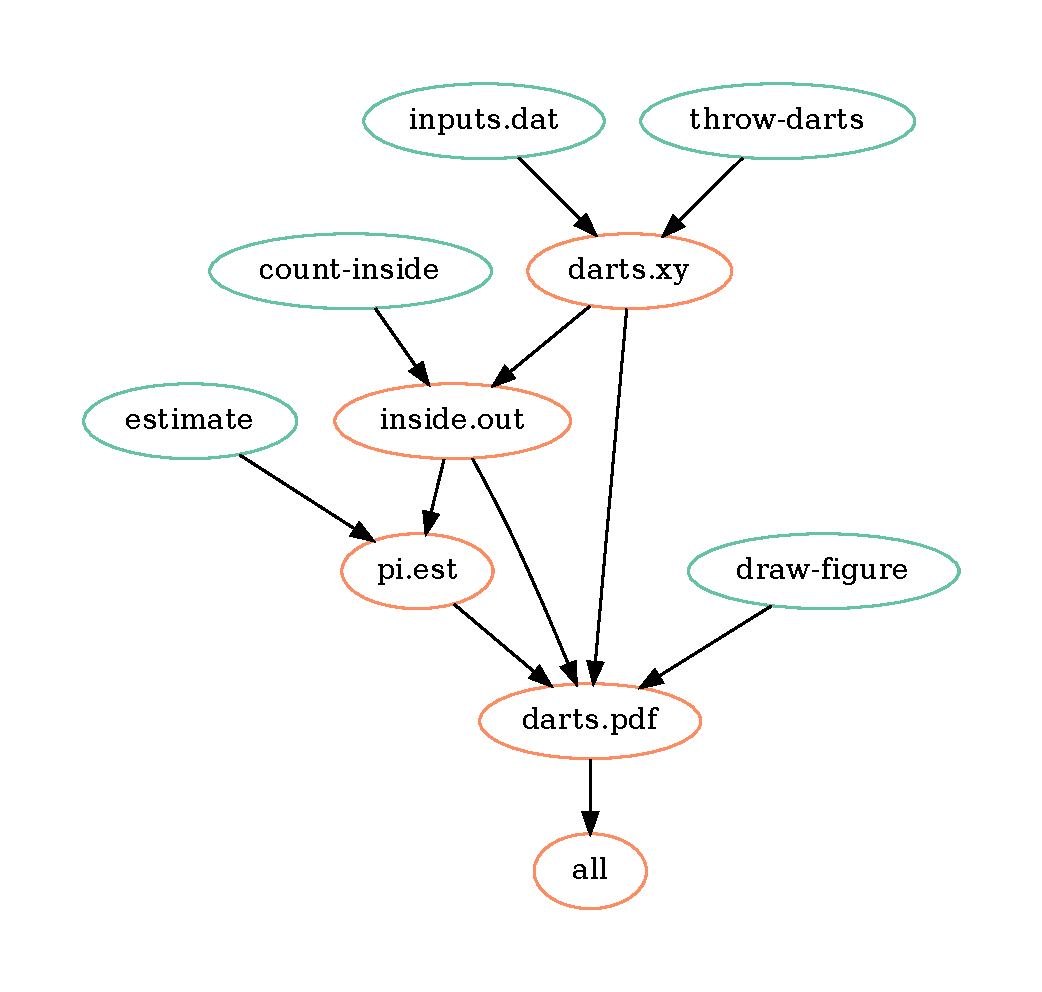
\includegraphics{v1-R/graph.pdf}
  \caption{DAG for Makefile version 1.  green ellipses correspond to
    those files that are up to date and do not need to be regenerated;
  red ellipsis are those files that need to be remade.}
  \label{fig:dag}
\end{figure}


(This figure is generated by analysing the structure of the output
from the make program, thanks to a program from \url{makefile2graph})

\subsection{Explain what PHONY targets are}

Two common PHONY targets are the "all" and "clean" targets.  "make
all" by convention is a request to regenerate all the files in the
directory, rather than to generate a file called "all".  Likewise,
"clean" is a convention to remove all the files that can be deleted.




\clearpage

\section{ersion 2 -- generate lots of simulations}

In version 2, we want to highlight how to make rules more flexible.
Example application here would be generating lots of simulation runs,
rather than just one.


\fbox{\lstinputlisting{v1-R/Makefile2}}

Try to generate B=15 samples, and then show a histogram of the
distribution of the B estimates of pi.


\begin{knitrout}
\definecolor{shadecolor}{rgb}{0.969, 0.969, 0.969}\color{fgcolor}\begin{kframe}
\begin{alltt}
cd v1-R
make -f Makefile2
cat pi-*est
\end{alltt}

\begin{verbatim}
## make[1]: Entering directory '/mhome/damtp/s/id318/Documents/Make_tutorial/make-tutorial/v1-R'
## ./throw-darts inputs.dat > darts-1.xy
## /bin/sh: 1: ./throw-darts: not found
## Makefile2:12: recipe for target 'darts-1.xy' failed
## make[1]: *** [darts-1.xy] Error 127
## rm darts-1.xy
## make[1]: Leaving directory '/mhome/damtp/s/id318/Documents/Make_tutorial/make-tutorial/v1-R'
## cat: 'pi-*est': No such file or directory
\end{verbatim}
\end{kframe}
\end{knitrout}


Describe make -j8 to run this in parallel.


NOTE: intermediate files are not kept.  

Perhaps show a 4x3 grid of 12 simulations?

\section{What next}

Further reading (books); other programs that build upon idea of make
(snakemake, drake).

\url{https://www.frontiersin.org/articles/10.3389/fninf.2016.00002/full}

Portable make code: \url{https://github.com/markpiffer/gmtt}


\subsection{Acknowledgements}

Mozilla CODECHECK for funding



\end{document}
